\subsection{LoadingSplashScreen}

Der Loading-Splash-Screen dient als zeitliche Überbrückung der Ladesequenz beim Starten der App und
wird solange angezeigt, bis der gespeicherte Session-Token validiert worden ist.

Wenn der gespeicherte Token gültig ist, wird der Nutzer auf die Hauptseite weitergeleitet. Andernfalls wird der Login- bzw. Signup-Screen angezeigt.

Da dieser Screen frei von Nutzer-Interaktion ist, wird dieser als Stateless Widget deklariert,
als Status-Anzeige wird ein \lstinline{CircularProgressIndicator}-Widget verwendet.

\begin{code}[H]
    \centering
    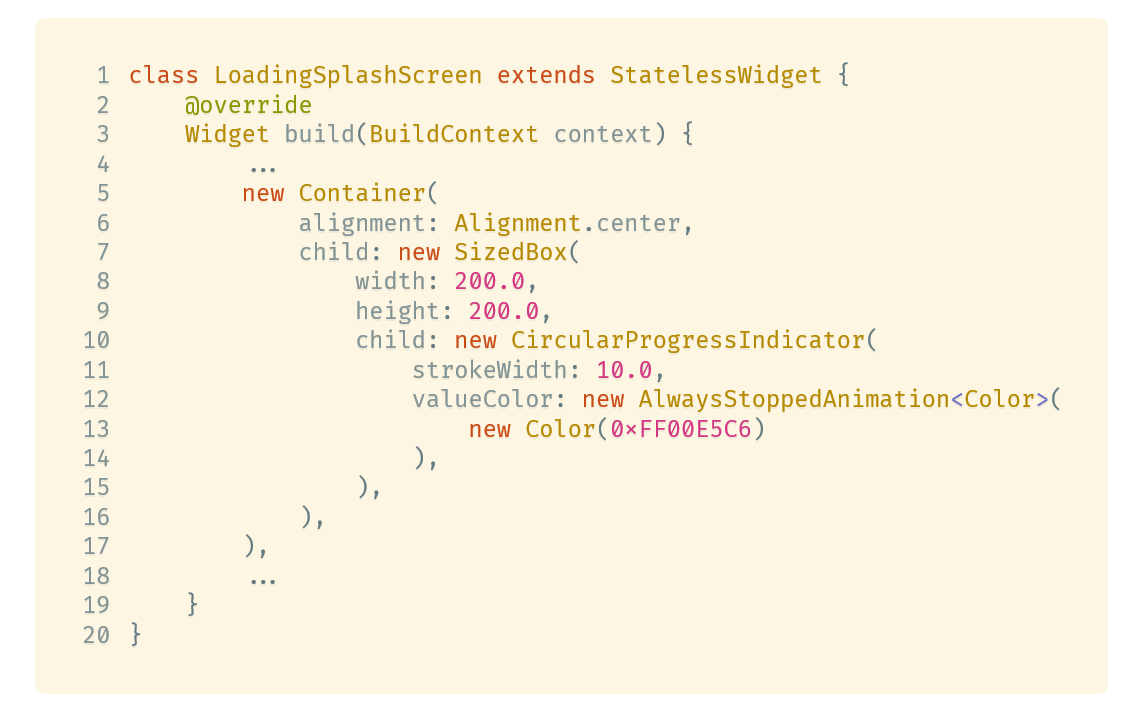
\includegraphics[width=1\textwidth]{images/Client/screens/loading/loadingWidget.png}
    \caption{Loading-Splash-Screen in Form eines Stateless Widgets}
\end{code}

\newpage

Dieser muss per MediaQuery als Alternativ-Route zu Login bzw. Signup und dem Home-Screen im App-Entry-Point
im \lstinline{main.dart}-File gesetzt werden.

\begin{code}[H]
    \centering
    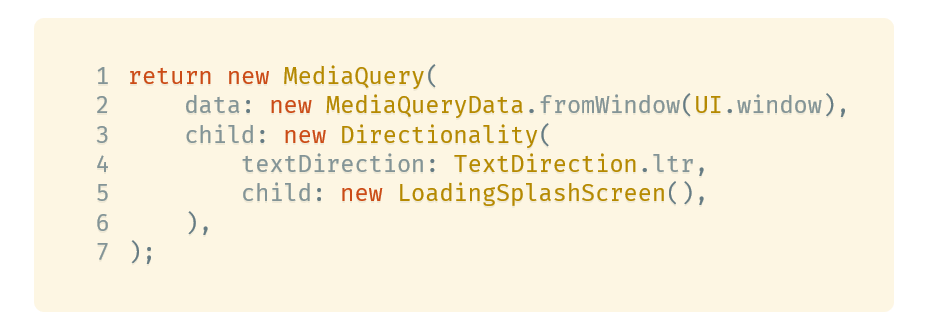
\includegraphics[width=1\textwidth]{images/Client/screens/loading/loadingScreen.png}
    \caption{Loading-Screen als Alternativ-Route per MediaQuery}
\end{code}